%Set the document class and font size
\documentclass[fleqn, bachelor,subf,12pt,notitlepage]{disser}

\usepackage[utf8]{inputenc}
\usepackage{enumerate}
\usepackage{amsmath}
\usepackage{mathtools} 
\usepackage{amssymb}
\usepackage{systeme}
\usepackage[english]{babel}
\usepackage{xparse}
\usepackage{xfrac}
\usepackage{setspace}
\usepackage{multicol}
\usepackage{array}
\usepackage{tabularx}
\usepackage{bigints}
\usepackage{fontspec}
\usepackage{fancyhdr}


%This is a command for creating new command for reducing the size of the given math equation
\newcommand\scalemath[2]{\scalebox{#1}{\mbox{\ensuremath{\displaystyle #2}}}}


\usepackage{geometry}
 \geometry
{
 	a4paper,
 	total={170mm,257mm},
 	left=30mm,
	right = 10mm,
 	top=20mm,
	bottom=25mm
 }

\pagestyle{fancy}
\fancyhead{}

\setmainfont{GHEA Grapalat}
\onehalfspacing

\title{Դիպլոմային աշխատանք}
\author{Կամո Սևոյան}
\date{}

\begin{document}
\section*{Ներածություն}
\subsection*{Հերմիթյան ինտերպոլյացիա}


Նախքան անդրադառնալը բազմաչամ ինտերպոլյացիայի խնդրին, քննարկենք մեկ փոփոխականի ֆունկցիայի ինտերպոլյացիայի որոշ դետալներ։ 

Ենթադրենք տրված են $f:A \mapsto B, A, B \subset \mathbb{R}$ ֆունկցիան,  $\left\{x_{i}\right\}_{i=0}^{N}$ կետերը և դրանց համապատասխան $\left\{y_{i}=f\left(x_{i}\right)\right\}_{i=0}^{N}$ արժեքները։ Յուրաքանչյուր $\left[x_{i}, x_{i+1}\right]$ հատվածում ինտերպոլացնող ֆունկցիան իրենից ներկայացնում է գխային ֆունկցիա, որը կարելի է ներկայացնել հետևյալ տեսքով.

$$p_{1}^{(i)}\left(x\right)=\dfrac{x_{i+1}-x}{x_{i+1}-x_{i}}y_{i}+\dfrac{x-x_{i+1}}{x_{i+1}-x_{i}}y_{i+1}, i=\overline{0, N-1}$$

Այսպիսով $\left[x_{0}, x_{N}\right]$ հատվածում կտոր առ կտոր մոտարկող ֆունկցիան տրվում է հետևյալ կերպ.

$$p_{1}\left(x\right)=\sum_{i=0}^{N}\varphi_{i} \left(x\right)y_{i}$$

Որտեղ 

\begin{align*}
\varphi_{0}\left(x\right)&=\begin{cases}
\dfrac{x_{1}-x}{x_{1}-x_{0}}, x\in \left[x_{0}, x_{1}\right]\\
0, x\in \left[x_{1}, x_{N}\right]\\
\end{cases}\\
\varphi_{i}\left(x\right)&=\begin{cases}
0, x\in \left[x_{0}, x_{i-1}\right]\\
\dfrac{x-x_{i-1}}{x_{i}-x_{i-1}}, x\in \left[x_{i-1}, x_{i}\right]\\
\dfrac{x_{i+1}-x}{x_{i+1}-x_{i}}, x\in \left[x_{i}, x_{i+1}\right]\\
0, x\in \left[x_{i+1}, x_{N}\right]\\
\end{cases}\\
\varphi_{N}\left(x\right)&=\begin{cases}
0, x\in \left[x_{0}, x_{N-1}\right]\\
\dfrac{x-x_{N-1}}{x_{N}-x_{N-1}}, x\in \left[x_{N-1}, x_{N}\right]\\
\end{cases}
\end{align*}

$\varphi_{i}\left(x\right)$ ֆունկցիաները կոչվում են բազիսային ֆունկցիաներ, որոնք ունեն այսպես կոչված լոկալ կրողներ, քանի որ դրանք ոչ զրոյական են որևէ տիրույթում և զրոյական որոշման տիրույթի մնացած մասերում։
Նմանատիպ բազիսային ֆունկցիաների հիմնական հատկությունն այն է, որ դրանք հավասար են մեկի որևէ կոնկրետ հանգույցում և հավասար են զրոյի մնացած բոլոր հանգույցներում։ Նշենք սակայն, որ այս տիպի ինտերպոլյացիան $C^{0}$ դասի է, այսինք միայն անընդհատ է, և հետևաբար կիրառելի չէ այն խնդիրներում, որտեղ պահանջվում է ավելի բարձր կարգի ողորկություն։


\newpage

Ստորև տրված է բազիսային ֆունկցիաների սխեմատիկ ներկայացում.
\begin{figure}[h!]
\centering
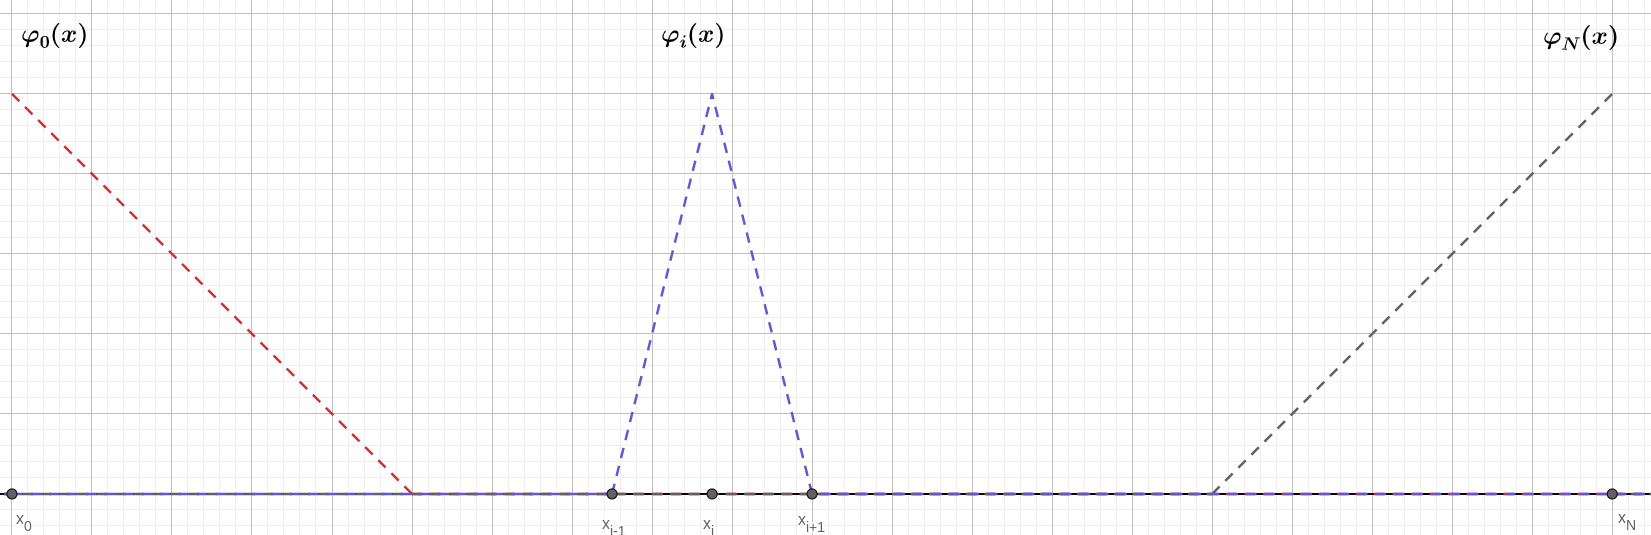
\includegraphics[width=1.0\textwidth]{images/image_1}
\captionsetup{labelformat=empty}
\caption{\hfill Նկար 1}
\end{figure}


\newpage

Այժմ դիտարկենք հետևյալ խնդիրը.
Անհրաժեշտ է կառուցել  կտոր առ կտեր մոտարկող ֆունկցիա, որը ֆունկցիայի արժեքի հետ մեկտեղ կհամըկնի նաև ֆունկցիայի առաջին կարգի ածանցյալի հետ ինտերպոլյացիոն կետերում։ Այսինքն.

$$ \dfrac{d^{j}}{dx^j}f(x_{i})=\dfrac{d^{j}}{dx^j}p_{3}(x_{i}),   \; j=0, 1;  \; i=\overline{0, N-1}$$

Յուրաքանչյուր $\left[x_{i}, x_{i+1}\right]$ հատվածում ինտերպոլյացիոն ֆունկցիան իրենից ներկայացնում է խորանարդային ֆունկցիա, որը կարելի է ներկայացնել հետևյալ տեսքով։

$$p_{3}^{\left(i\right)} = \alpha_{i}(x)f(x_{i})+\beta_{i+1}(x)f(x_{i+1})+\gamma_{i}(x)f^{'}(x_{i})+\delta_{i+1}(x)f^{'}(x_{i+1})$$

որտեղ 

$$\alpha_{i}(x)=\dfrac{\left(x_{i+1}-x\right)^{2}\left[\left(x_{i+1}-x_{i}\right)+2\left(x-x_{i}\right)\right]}{\left(x_{i+1}-x_{i}\right)^{3}}, \beta_{i+1}(x)=\dfrac{\left(x-x_{i}\right)^{2}\left[\left(x_{i+1}-x_{i}\right)+2\left(x_{i+1}-x\right)\right]}{\left(x_{i+1}-x_{i}\right)^{3}}$$

$$\gamma_{i}(x)=\dfrac{\left(x-x_{i}\right)\left(x_{i+1}-x\right)^{2}}{\left(x_{i+1}-x_{i}\right)^{2}}, \delta_{i+1}(x)=\dfrac{\left(x-x_{i}\right)^2\left(x-x_{i+1}\right)}{\left(x_{i+1}-x_{i}\right)^{2}}$$

Այսպիսով $\left[x_{0}, x_{N}\right]$ հատվածում կտոր առ կտոր մոտարկող ֆունկցիան տրվում է հետևյալ կերպ.

$$p_{3}(x)=\sum_{i=0}^{N}\left[\varphi_{i}^{(0)}f(x_{i})+\varphi_{i}^{(1)}f^{'}(x_{i})\right]$$
որտեղ 
\begin{align*}
\varphi^{(0)}_{0}\left(x\right)&=\begin{cases}
\dfrac{\left(x_{1}-x\right)^{2}\left[\left(x_{1}-x_{0}\right)+2\left(x-x_{0}\right)\right]}{\left(x_{1}-x_{0}\right)^{3}},  x\in \left[x_{0}, x_{1}\right]\\
0, x\in \left[x_{1}, x_{N}\right]\\
\end{cases}\\
\varphi^{(0)}_{i}\left(x\right)&=\begin{cases}
0, x\in \left[x_{0}, x_{i-1}\right]\\
\dfrac{\left(x-x_{i-1}\right)^{2}\left[\left(x_{i}-x_{i-1}\right)+2\left(x_{i}-x\right)\right]}{\left(x_{i}-x_{i-1}\right)^{3}}, x\in \left[x_{i-1}, x_{i}\right]\\
\dfrac{\left(x_{i+1}-x\right)^{2}\left[\left(x_{i+1}-x_{i}\right)+2\left(x-x_{i}\right)\right]}{\left(x_{i+1}-x_{i}\right)^{3}}, x\in \left[x_{i}, x_{i+1}\right]\\
0, x\in \left[x_{i+1}, x_{N}\right]\\
\end{cases}\\
\varphi^{(0)}_{N}\left(x\right)&=\begin{cases}
0, x\in \left[x_{0}, x_{N-1}\right]\\
\dfrac{\left(x-x_{N-1}\right)^{2}\left[\left(x_{N}-x_{N-1}\right)+2\left(x_{N}-x\right)\right]}{\left(x_{N}-x_{N-1}\right)^{3}}, x\in \left[x_{N-1}, x_{N}\right]\\
\end{cases}
\end{align*}

\begin{align*}
\varphi^{(1)}_{0}\left(x\right)&=\begin{cases}
\dfrac{\left(x-x_{0}\right)\left(x_{1}-x\right)^{2}}{\left(x_{1}-x_{0}\right)^{2}}, x\in \left[x_{0}, x_{1}\right]\\
0, x\in \left[x_{1}, x_{N}\right]\\
\end{cases}\\
\varphi^{(1)}_{i}\left(x\right)&=\begin{cases}
0, x\in \left[x_{0}, x_{i-1}\right]\\
\dfrac{\left(x-x_{i-1}\right)^2\left(x-x_{i}\right)}{\left(x_{i}-x_{i-1}\right)^{2}}, x\in \left[x_{i-1}, x_{i}\right]\\
\dfrac{\left(x-x_{i}\right)\left(x_{i+1}-x\right)^{2}}{\left(x_{i+1}-x_{i}\right)^{2}}, x\in \left[x_{i}, x_{i+1}\right]\\
0, x\in \left[x_{i+1}, x_{N}\right]\\
\end{cases}\\
\varphi^{(1)}_{N}\left(x\right)&=\begin{cases}
0, x\in \left[x_{0}, x_{N-1}\right]\\
\dfrac{\left(x-x_{N-1}\right)^{2}\left(x-x_{N}\right)}{\left(x_{N}-x_{N-1}\right)^{2}}, x\in \left[x_{N-1}, x_{N}\right]\\
\end{cases}
\end{align*}

Ստորև տրված է բազիսային ֆունկցիաների սխեմատիկ ներկայացում.
\begin{figure}[h!]
\centering
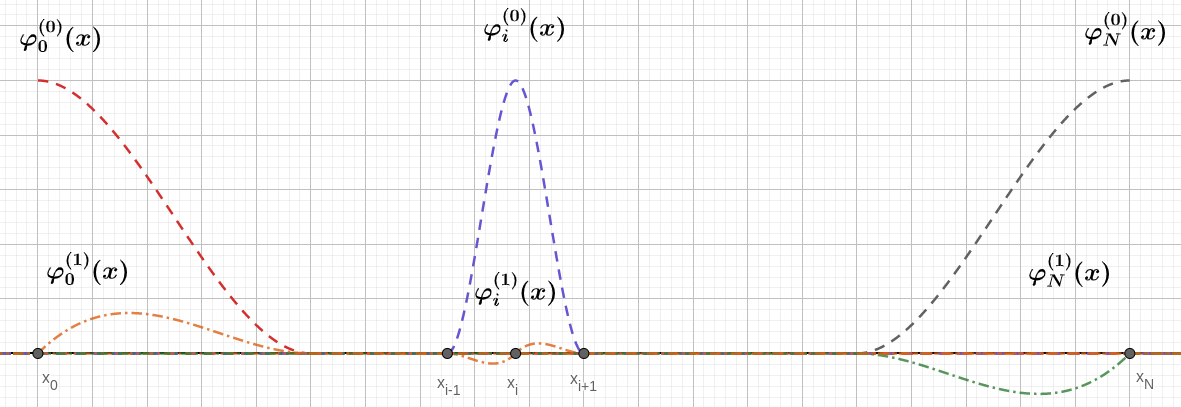
\includegraphics[width=1.0\textwidth]{images/image_2}
\captionsetup{labelformat=empty}
\caption{\hfill Նկար 2}
\end{figure}

Այսպիսով ստացանք $C^{1}$ ինտերպոլյացիա։

Ընդհանուր դեպքում հերմիթյան ինտերպոլյացիայի պայմանը կարելի է գրել հետևյալ կերպ.
$$\dfrac{d^{k}}{dx^{k}}f\left(x_{i}\right)=\dfrac{d^{k}}{dx^{k}}p_{2m-1}\left(x_{i}\right), \;  i=\overline{0, N}, \;  k=\overline{0, m-1}$$

\newpage

\subsection*{Խորանարդային ինտերպոլյացիա}

Խնդիրներում, որտեղ անհրաժեշտ է որոշել միայն տրված ֆունկիցիան, ֆունկցիայի ածանցյալներն ինտերպոլացնելու փոխարեն դրվում է դրանց անընդհատության պայման բազիսային ֆուկցիաների միացման կետերում,  բավականին հեշտացնելով դրված խնդիրը և դրա լուծումը։ Սակայն այս դեպքում բազիսային ֆունկցիաները չեն հանդիսանում լոկալ կրողներ, ուստի կիրառական տեսանկյունից հարմար չեն։

Նման տիպի ինտերպոլյացիայի կառուցման պարզագույն օրինակը հետևյալն է.

\noindent Յուրաքանչյուր $\left[x_{i}, x_{i+1}\right]$ ինտերվալում կառուցենք այպիսի պարաբոլ, որ բոլոր $x_{i}$ հանգուցային կետերում առանջին կարգի ածանցյալները լինեն անընդհատ։

$$S_{2}^{(i)}(x)=f(x_{i})+\dfrac{f(x_{i+1})-f(x_{i})}{x_{i+1}-x_{i}}\left(x-x_{i}\right)+c_{i}\left(x-x_{i}\right)\left(x-x_{i+1}\right)$$

\noindent Ածանցյալների անընդհատության պայմանից կհետևի, որ

$$c_{i}+c_{i-1}=\dfrac{1}{h^{2}}\left(f(x_{i+1})-2f(x_{i})+f(x_{i-1})\right) \; i=\overline{1, N-1}$$

Քանի որ համակարը պարունակում է $N-1$ հավասարում, ապա մնում է մեկ ազատ գործակից, որը կարելի գտնել, որևէ $x_{j}$ հանգուցային կետում որոշելով $S_{2}^{(j)''}$֊ն։
%TODO: Add some equations and a plot

\begin{figure}[h!]
\centering
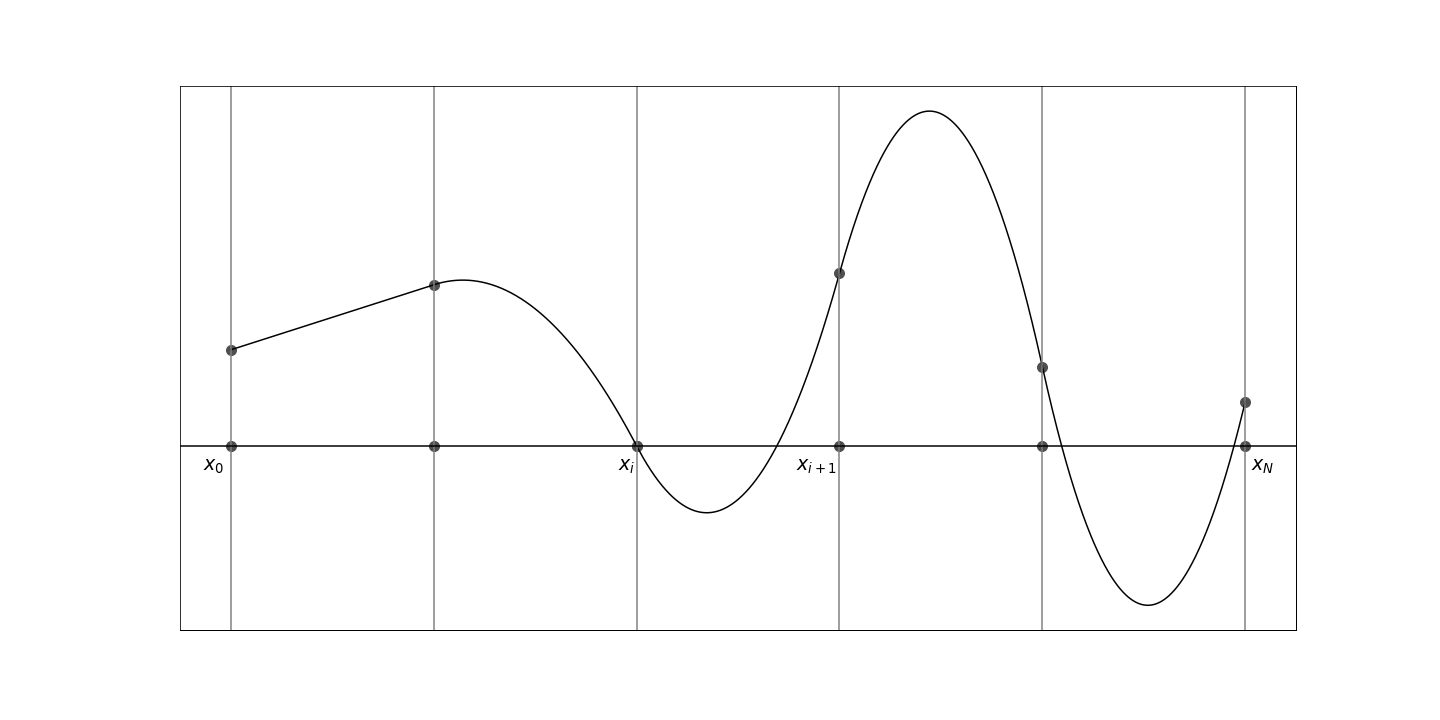
\includegraphics[width=1.0\textwidth]{images/image_8}
\captionsetup{labelformat=empty}
\caption{\hfill Նկար 3}
\end{figure}

Առավել կիրառելի են խորանարդային սփլայնները։ Այս դեպքում յուրաքանչյուր $\left[x_{i}, x_{i+1}\right]$ ինտերվալում կառուցվում են երրորդ աստիճանի բազմանդամներ այնպիսին, որ դրանց միացման կետերում (հանգույցներում) առաջին և երկրորդ կարգի ածանցյալները լինեն անընդհատ։ 

Բազմանդամը դիտարկելու փոխարեն դիտարկենք նրա երկրորդ կարգի ածանցյալը: Այն գծային ֆունկցիա է, հետևաբար այն կարելի է ներկայացնել հետևյալ տեսքով.

$$ S^{(i)''}_3(x)=c_{i}\dfrac{x_{i+1}-x}{x-x_{i}}+c_{i+1}\dfrac{x-x_{i}}{x_{i+1}-x_{i}}$$



\newpage
\section*{Երկչափ մոտարկում}

Այժմ դիտարկենք երկու փոփոխականի կտոր առ կտոր անընդհատ մոտարկման խնդիրը $\partial R$ եզրով սահմանափակ $R$ տիրությում։ Տիրույթը տրոհվում է որոշակի թվով էլեմենտների։ Կախված $R$ տիրույթից, առանձնացվում են հետևյալ մոտակման ձևերը.

\subsection*{Ուղղանկյուն տիրույթ}
\subsubsection*{$C^{(0,0)}$ մոտարկում}

Դիցուք տրված են $f:\Omega\mapsto B$,  $B \subset \mathbb{R}$, $\Omega \subset \mathbb{R}^{2} = \left[x_{0}, x_{M}\right] \times \left[y_{0}, y_{M}\right]$,  ուղղանկյուն տիրույթը, որը տրոհված է $\left[x_{i}, x_{i+1}\right] \times \left[y_{j}, y_{j+1}\right]$, ուղղանկյուն էլեմենտների:
$$x_{i+1}-x_{i}=h_{1}, \; y_{j+1}-y_{j}=h_{2}, \; i=\overline{0, M-1}, j=\overline{0, N-1}$$

\begin{figure}[h!]
\centering
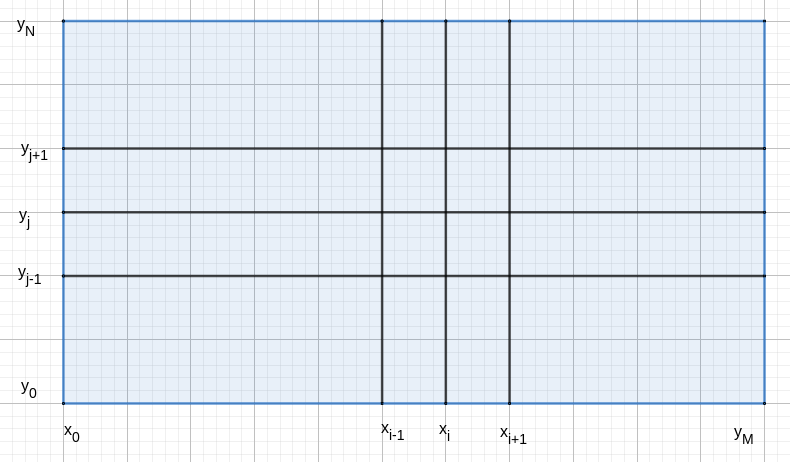
\includegraphics[width=0.6\textwidth]{images/image_3}
\captionsetup{labelformat=empty}
\caption{\hfill Նկար 3}
\end{figure}

Յուրաքանչյուր  $\left[x_{i}, x_{i+1}\right] \times \left[y_{j}, y_{j+1}\right]$ էլեմենտի վրա $f$ ֆունկցիան մոտարկվում հետևյալ քառակուսային ֆունկցիայով։

$$\scalemath{0.9}{p_{1}^{(i, j)}(x, y)=\alpha_{i,j}(x,y)f(x_{i},y_{j})+\beta_{i+1,j}(x,y)f(x_{i+1},y_{j})\scalemath{0.2}+\gamma_{i,j+1}(x,y) f(x_{i},y_{j+1})+\delta_{i+1, j+1}(x,y)f(x_{i+1},y_{j+1})}$$
 որտեղ 

$$\alpha_{i,j}(x,y)=\dfrac{1}{h_{1}h_{2}}\left(x_{i+1}-x\right)\left(y_{j+1}-y\right)$$
$$\beta_{i+1,j}(x,y)=\dfrac{1}{h_{1}h_{2}}\left(x-x_{i}\right)\left(y_{j+1}-y\right)$$
$$\gamma_{i,j+1}(x,y)=\dfrac{1}{h_{1}h_{2}}\left(x_{i+1}-x\right)\left(y-y_{j}\right)$$
$$\delta_{i+,j+1}(x,y)=\dfrac{1}{h_{1}h_{2}}\left(x-x_{i}\right)\left(y-y_{j}\right)$$

Այսպիսով $\left[x_{0}, x_{M}\right] \times \left[y_{0}, y_{M}\right]$ տիրույթում կտոր առ կտոր մոտարկող ֆունկցիան տրվում է հետևյալ կերպ.

$$p_{1}(x,y)=\sum_{i=0}^{m}\sum_{j=0}^{n}\varphi_{i,j}(x,y)f(x_{i},y_{j})$$
որտեղ

%TODO: change 'otherwise' to armenian one, at this moment this is not possible because XeLaTeX can not render armenian letter in math equations

$$\varphi_{i,j}\left(x, y\right)=\begin{cases}
\frac{1}{h_{1}h_{2}}\left(x-x_{i-1}\right)\left(y-y_{j-1}\right), (x,y)\in \left[x_{i-1}, x_{i}\right]\times\left[y_{j-1}, y_{j}\right]\\
\frac{1}{h_{1}h_{2}}\left(x-x_{i-1}\right)\left(y_{j+1}-y\right), (x,y)\in \left[x_{i-1}, x_{i}\right]\times\left[y_{j}, y_{j+1}\right]\\
\frac{1}{h_{1}h_{2}}\left(x_{i+1}-x\right)\left(y-y_{j-1}\right), (x,y)\in \left[x_{i}, x_{i+1}\right]\times\left[y_{j-1}, y_{j}\right]\\
\frac{1}{h_{1}h_{2}}\left(x_{i+1}-x\right)\left(y_{j+1}-y\right), (x,y)\in \left[x_{i}, x_{i+1}\right]\times\left[y_{j}, y_{j+1}\right]\\
0, otherwise\\
\end{cases}$$

Վերը դիտարկված մոտարկումը հանդիսանում է երկչափ Հերմիթյան մոտարկման մասնավոր դեպք։

Ընդհանուր դեպքում, տրված $k\in \mathbb{N}$ թվի և տրված ուղղանկյուն տիրույթի ցանկացած ուղղանկյունաձև տրոհման էլեմենտում կարելի է կառուցել $C^{k-1, k-1}$ կարգի մոտարկող բազմանդամ, որը $2k-1$ ֊րդ կարգի բազմանդամ է ըստ իր յուրաքանչյուր փոփոխականի և, ինտերպոլյացիայի պայմանները կարելի է գրել հետևյալ կերպ.

$$ \dfrac{d^{p+q}}{dx^p dy^{q}}f(x_{i}, y_{j})=\dfrac{d^{p+q}}{dx^{p}dy^{q}}p_{2k-1}(x_{i}, y_{j})$$
$$p, q = \overline{0, k-1}; \; i=\overline{0, M};  \;  j=\overline{0, N}$$


\newpage

\noindent Այժմ դիտարկենք ուղղանկյուն տիրույթի տրոհման և բազիսային ֆունկցիաների կառուցման այլ տարբերակ։ Այս դեպքում տիրույթը տրոհենք ըստ նախորդ տարբերակի, ի հավելումն յուրաքանչյուր ուղղանկյուն էլեմենտ տրոհելով երկու ուղղանկյուն եռանկյունների.

Դիտարկենք հետևյալ ֆունկցիան.

$$\varphi \left(x,y\right)=\begin{cases}
1-y, &(x,y) \in S_{1} \\
1-x+y, &(x,y) \in S_{2} \\
1+x, &(x,y) \in S_{3} \\
1+y, &(x,y) \in S_{4} \\
1-x+y, &(x,y) \in S_{5} \\
1-x, &(x,y) \in S_{6}\\
0, otherwise
\end{cases} $$


\begin{figure}[h!]
  \centering
  \begin{minipage}[b]{0.4\textwidth}
    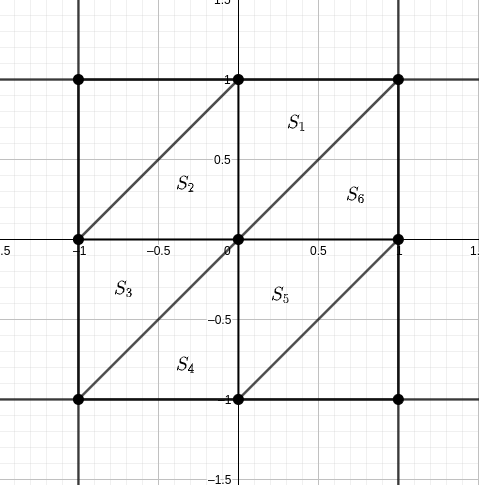
\includegraphics[width=\textwidth]{images/image_4.png}
    \captionsetup{labelformat=empty}
    \caption{Նկար 4}
  \end{minipage}
  \hfill
  \begin{minipage}[b]{0.4\textwidth}
    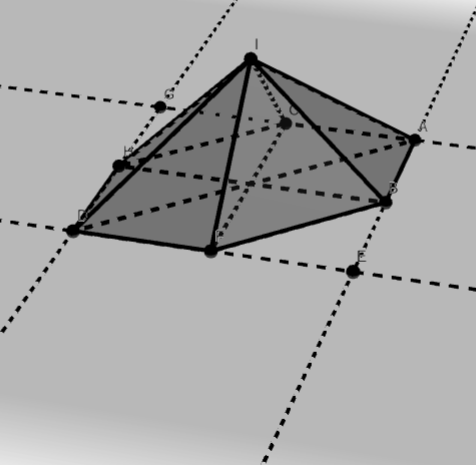
\includegraphics[width=\textwidth]{images/image_6.png}
    \captionsetup{labelformat=empty}
    \caption{Նկար 5}
  \end{minipage}
\end{figure}

\noindent Պարզ է, որ այն յուրաքանչյուր ուղղանկյուն էլեմենտում $C^{(0, 0)}$ ֆունկցիա է:

\noindent  Այժմ յուրաքանչյուր $x_{i}, y_{j}$ կետի վրա կառուցենք հետևյալ ֆունկցիան.

$$\varphi_{i,j}(x,y)=\varphi \left(\dfrac{x-x_{i}}{h_{1}}, \dfrac{y-y_{j}}{h_{2}}\right)$$

\newpage

Այդ դեպքում $f$ ֆունկցիայի մոտարկման բանաձևը կտվրի հետևյալ կերպ։

$$p_{1}(x,y)=\sum_{i=0}^{N}\sum_{j=0}^{M}\varphi_{i,j}(x,y)f(x_{i}, y_{j})$$

\begin{figure}[h!]
\centering
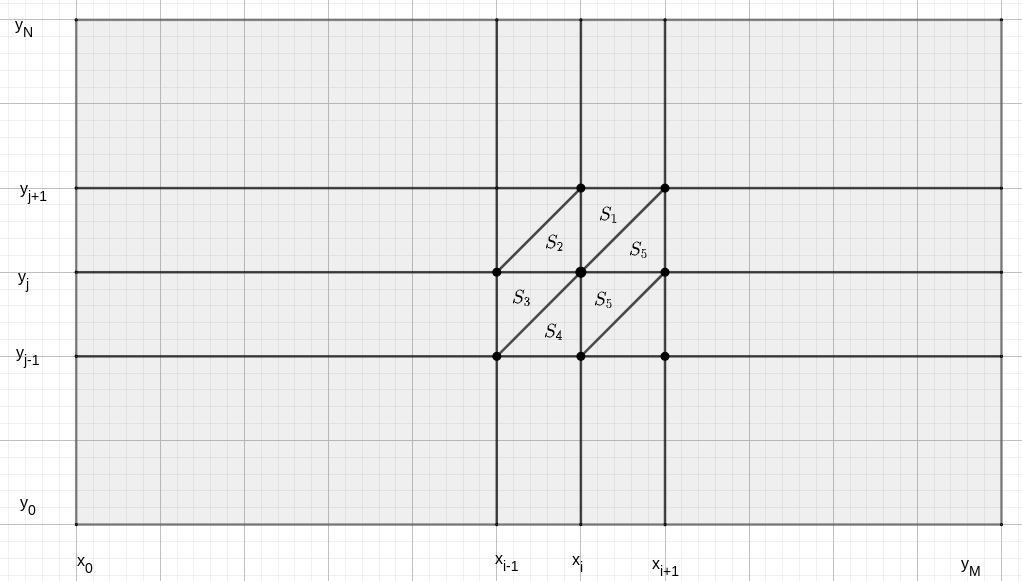
\includegraphics[width=0.6\textwidth]{images/image_5}
\captionsetup{labelformat=empty}
\caption{\hfill Նկար 5}
\end{figure}

\newpage

\subsection*{Բազմանկյուն տիրույթ}

Բազմանկյուն տիրույթ ասելով կհասկանանք կամ հենց բազմանկյունաձև տիրույթը, կամ դրա՝ բազմանկյունով մոտարկումը։ 

Դիցուք տրված են $f:\Omega\mapsto B$,  $B \subset \mathbb{R}$, $\Omega \subset \mathbb{R}^{2} $ բազմանկյուն տիրույթը, որը կամայական ձևով տրոհված է եռանկյուն էլեմենտների։ Յուրաքանչյուր այդպիսի $P_{1}, P_{2}, P_{3}$ գագաթներով եռանկյան համար դիտարկենք հետևյալ մոտարկող ֆունկցիան.

$$p_{1}(x, y) = \dfrac{1}{S}\sum_{i=1}^{3} p^{(1)}_{i}(x,y)f(x_{i}, y_{i})$$

$$S = \begin{vmatrix}
     1 & x_1 & y_1\\ 
     1 & x_2 & y_2\\
     1 & x_3 & y_3 
\end{vmatrix}$$

$$p^{(1)}_{i}(x,y) = x_{j}y_{k}-x_{k}y_{j}+x(y_{j}-y_{k})-y(x_{j}-x_{k})$$

\noindent որտեղ $(x_{i}, y_{i}), \; i=1, 2, 3$ տրված եռանկյուն էլեմենտի գագաթներն են (հերթականությունը ժամսլաքին հակառակ ուղղությամբ)։

\begin{figure}[h!]
\centering
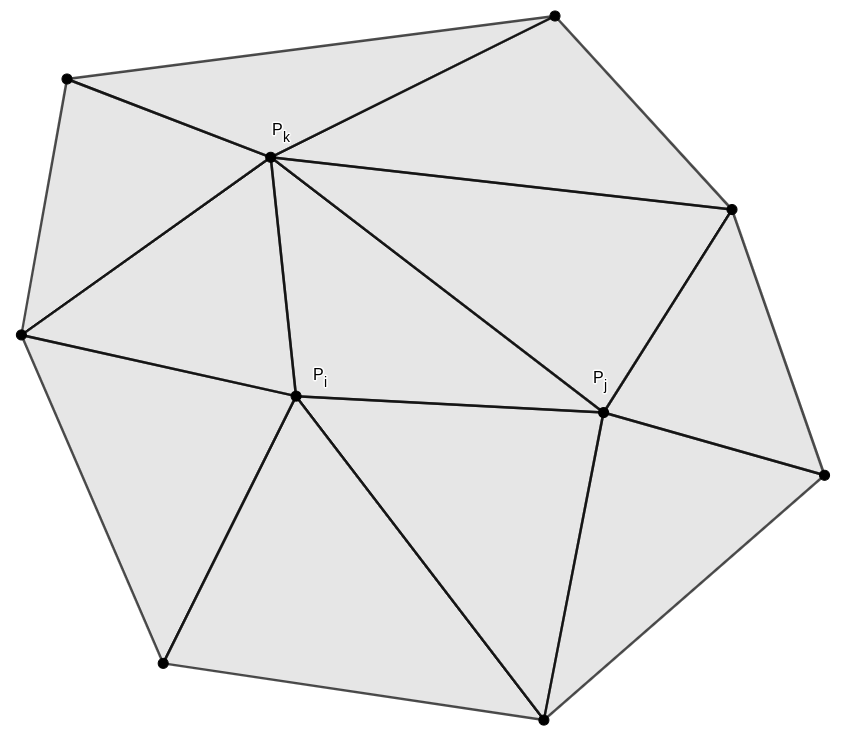
\includegraphics[width=0.4\textwidth]{images/image_7}
\captionsetup{labelformat=empty}
\caption{\hfill Նկար 6}
\end{figure}

\noindent Բնական է, որ որևէ կետի նկատմամբ լրիվ բազիսային ֆունկցիայի կառուցելու համար անհրաժեշտ է իրար գումարել այն բոլոր եռանկյուն էլեմենտների՝ այդ կետին համապատասխան ֆունկցիաները, որոնց համար տվյալ կետը գագաթ է։ Հետևաբար, ընդհանուր դեպքում վերը նշված մոտարկան եղանակը հաշվողական տեսակետից հարմար չէ։

\newpage
\section*{Վարիացիոն մեթոդ}

Վարիացիոն մեթոդները հանդիպում են բազմաթիվ ֆիզիկական և այլ խնդիրնորում, և այդ խնդիրների մոտավոր լուծումը հիմնված է համապատասխան վարիացիոն մեթոդներին։


\end{document}